% !TEX spellcheck = fr_FR

%%%% Paramétrage du cours %%%%
\def\xxactivite{Cours}

\def\xxauteur{Emilien Durif -- Xavier Pessoles}
\fichefalse \proftrue \tdfalse \courstrue

\def\xxnumchapitre{Chapitre 7 \vspace{.2cm}}

\def\xxchapitre{Complexité algorithmique }

\def\xxcompetences{%
\textsl{%
\textbf{Savoirs et compétences :}\\
\begin{itemize}[label=\ding{112},font=\color{bleuxp}] 
\item Complexité.
\end{itemize}
}}

\def\xxfigures{
%
\includegraphics[width=\linewidth]{fractale}
%\\
%\textit{Modèle du pilote hydraulique avec pilotage interactif.}
}%figues de la page de garde

\input{\repRel/Style/pagegarde_cours_minitoc}
\setlength{\columnseprule}{.1pt}

\vspace{2cm}
\pagestyle{fancy}
\thispagestyle{plain}
%%%%%%%%%%%%%%%%%%%%%%%
\section{Mise en évidence du problème}

%\subsection{Premier exemple}
%On introduit les algorithmes de tri suivant : 
%\begin{py}
%\begin{python}
%#Tri par sélection
%def tri_selection(tab):
%    for i in range(0,len(tab)):
%        indice = i
%        for j in range(i+1,len(tab)):
%            if tab[j]<tab[indice]:
%               indice = j
%        tab[i],tab[indice]=tab[indice],tab[i]
%    return tab
%\end{python}
%\end{py}
%
%\begin{py}
%\begin{python}    
%#Tri par insertion
%def tri_insertion(tab):
%    for i in range(1,len(tab)):
%        a=tab[i] 
%        j=i-1    
%        while j>=0 and tab[j]>a:
%            tab[j+1]=tab[j]
%            j=j-1
%        tab[j+1]=a
%    return tab
%\end{python}
%\end{py}
%
%\begin{py}
%\begin{python}
%def shellSort(array):
%     "Shell sort using Shell's (original) gap sequence: n/2, n/4, ..., 1."
%     "http://en.wikibooks.org/wiki/Algorithm_Implementation/Sorting/Shell_sort#Python"
%     gap = len(array) // 2
%     # loop over the gaps
%     while gap > 0:
%         # do the insertion sort
%         for i in range(gap, len(array)):
%             val = array[i]
%             j = i
%             while j >= gap and array[j - gap] > val:
%                 array[j] = array[j - gap]
%                 j -= gap
%             array[j] = val
%         gap //= 2
%\end{python}
%\end{py}
%
%La figure ci-dessous montre le temps en secondes pour trier des tableaux de 1 à 1000 éléments en utilisant les méthodes de tri suivant : 
%\begin{itemize}
%\item tri par sélection;
%\item tri par insertion; 
%\item tri shell;
%\item méthode de tri utilisée par Python.
%\end{itemize}
%
%Le premier graphe montre le temps de calcul et le second une estimation du nombre d'opérations. 
%
%\begin{minipage}[c]{.48\linewidth}
%\begin{center}
%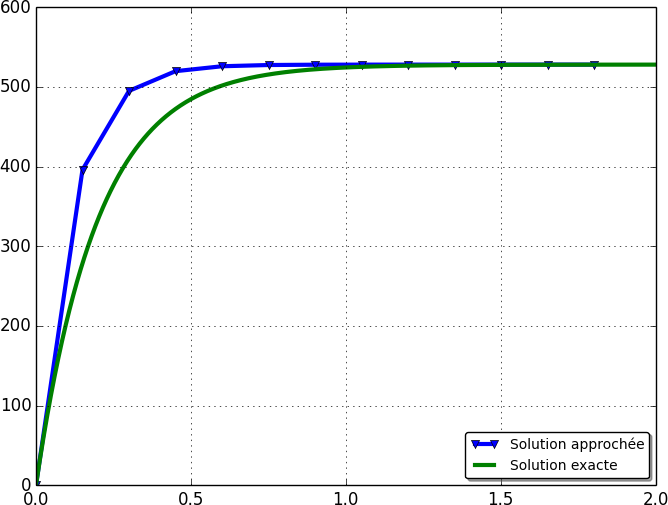
\includegraphics[width=.95\textwidth]{figure_1}
%\end{center}
%\end{minipage}\hfill
%\begin{minipage}[c]{.48\linewidth}
%\begin{center}
%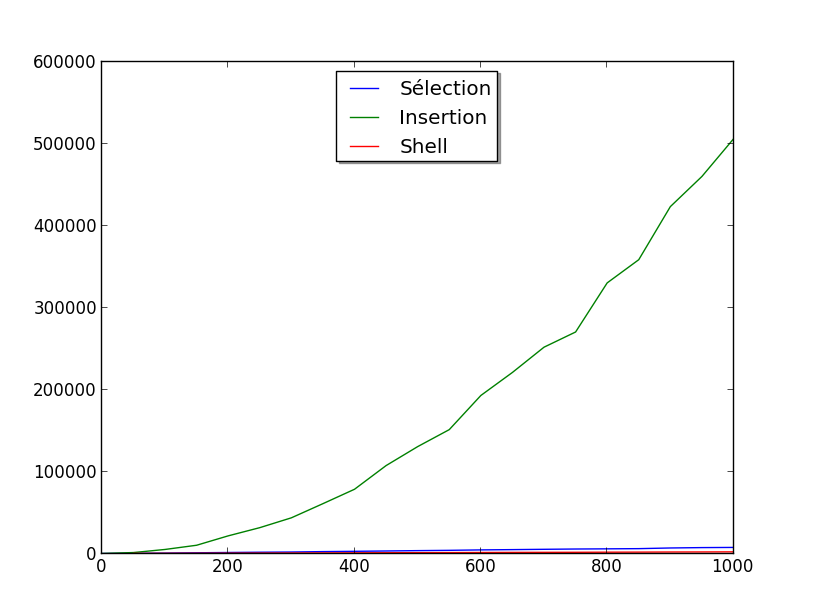
\includegraphics[width=.95\textwidth]{figure_2}
%\end{center}
%\end{minipage}

%\subsection{Deuxième exemple}
Prienons l'exemple de la recherche d'un élément dans une liste : 


\noindent
\begin{minipage}[c]{.49\linewidth}
%
%\begin{pseudo}
%\begin{center}
%\begin{tabular}{p{.9\textwidth}}
%\hline
%\textbf{Algorithme :} Recherche d'un nombre dans une liste triée ou non \\
%\hline
%\textbf{Données :}
%\begin{itemize}
%\item \texttt{nb}, int : un entier 
%\item \texttt{tab}, liste : une liste d'entiers triés ou non triés
%\end{itemize}
%\textbf{Résultat :} un booléen : \texttt{Vrai} si le nombre est dans la liste, \texttt{Faux} sinon. \\
%\\
%\textbf{is\_number\_in\_list}(\texttt{nb},\texttt{tab}) :\\
%\hspace{.4cm}\texttt{l} $\leftarrow$ \textbf{longueur}(\texttt{tab}) \\
%\hspace{.4cm}\textbf{Pour} \texttt{i} \textbf{allant de} 1 \textbf{à} \texttt{l} \textbf{faire} : \\
%\hspace{.8cm} \textbf{Si}  \texttt{tab[i] = nb} \textbf{alors} :\\
%\hspace{1.2cm}\textbf{Retourne} \texttt{Vrai} \\
%\hspace{.8cm} \textbf{Fin Si} \\
%\hspace{.4cm}\textbf{Fin Faire} \\
%\hspace{.4cm}\textbf{Retourne} \texttt{Faux} \\
%\textbf{Fin fonction} \\
%\hline
%\end{tabular}
%\end{center}
%\end{pseudo}

\begin{lstlisting}
def is_number_in_list(nb,tab):
    """Renvoie True si le nombre nb est dans la liste de nombres tab
    Entrées :
      * nb, int -- nombre entier
      * tab, list -- liste de nombres entiers    
    """
    for i in range(len(tab)):
        if tab[i]==nb:
            return True
    return False
\end{lstlisting}


\begin{exemple}
\`A partir de l'algorithme précédent, évaluer : 
\begin{itemize}
\item le nombre de tour de boucles dans le pire des cas;
\item le nombre de tour de boucles dans le meilleur des cas.
\end{itemize}
\end{exemple}

\end{minipage}\hfill
\begin{minipage}[c]{.49\linewidth}
\begin{lstlisting}
def is_number_in_list_dicho(nb,tab):
    """ 
    Recherche d'un nombre par dichotomie dans un tableau trié. 
    Renvoie l'index si le nombre nb est dans la liste de nombres tab.
    Renvoie None sinon.
    Entrées :
     * nb,int -- nombre entier
     * tab,list -- liste de nombres entiers triés
    """
    g, d = 0, len(tab)-1
    while g <= d:
        m = (g + d) // 2
        if tab[m] == nb:
            return m
        if tab[m] < nb:
            g = m+1
        else:
            d = m-1
    return None
\end{lstlisting}



\end{minipage}






\begin{center}
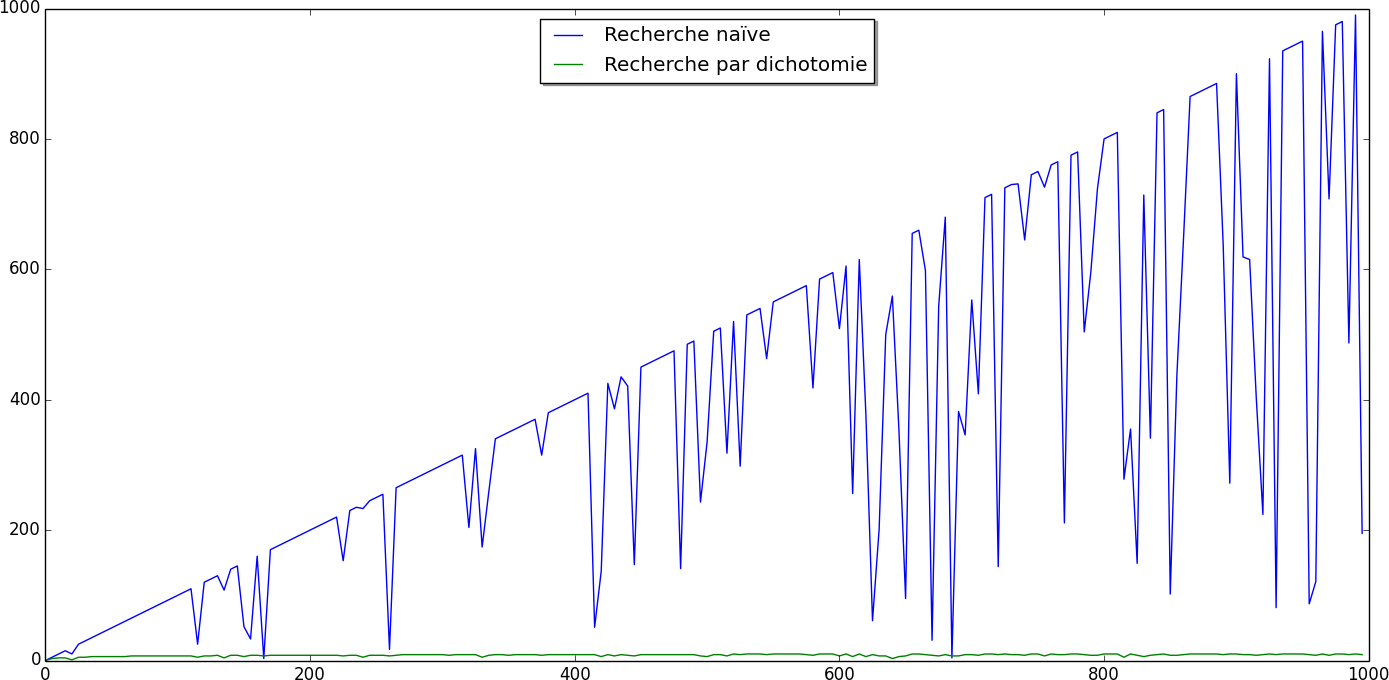
\includegraphics[width=.95\textwidth]{figure_5}

\textit{Évolution du nombre d'opérations pour rechercher un nombre dans une liste de 1 à 1000 nombres}
\end{center}



\section{Complexité des algorithmes}

\subsection{Présentation}
Il existe souvent plusieurs façons de programmer un algorithme. Si le nombre d'opérations à effectuer est peu important et les données d'entrée de l'algorithme sont de faibles tailles, le choix de la solution importe peu. En revanche, lorsque le nombre d'opérations et la taille des données d'entrée deviennent importants, deux paramètres deviennent déterminants : le temps d'exécution et l'occupation mémoire. 


\begin{defi}{Complexité en temps}

La complexité en temps donne le nombre d'opérations effectuées lors de l'exécution d'un programme. On appelle $C_o$ le coût en temps d'une opération $o$.

\end{defi}

\begin{defi}{Complexité en mémoire (ou en espace)}

La complexité en mémoire donne le nombre d'emplacements mémoires occupés lors de l'exécution d'un programme.
\end{defi}

\begin{rem}

On distingue la complexité dans le pire des cas, la complexité dans le meilleure des cas, ou la complexité en moyenne. En effet, pour un même algorithme, suivant les données à manipuler, le résultat sera déterminé plus ou moins rapidement. 

Généralement, on s'intéresse au cas le plus défavorable à savoir, la complexité dans le pire des cas. 
\end{rem}

\begin{defi}{Complexité algorithmique -- Notation $\mathcal{O}$}
 [Bournez]
Soient $f$ et $g$ deux fonctions $f,g : \mathbb{N} \rightarrow \mathbb{R}^{+}_{*}$. On note $f(n)=\mathcal{O}(g(n))$ lorsqu'il existe $c\in\mathbb{R}^+$ et $n_0\in\mathbb{N}$ tels que pour tout $n\geq n_0$, 
$$
f(n) \leq c\cdot g(n)
$$

Intuitivement, cela signifie que $f$ est inférieur à $g$ à une constante multiplicative près pour les données suffisamment grandes. 

\end{defi}

\begin{exemple}
Par ordre de complexité croissante on a :
\begin{itemize}
\item $\mathcal{O}(1)$ : algorithme s'exécutant en temps constant, quelle que soit la taille des données;
\item $\mathcal{O}(\log(n))$ : algorithme rapide (complexité logarithmique) (Exemple : recherche par dichotomie dans un tableau trié);
\item $\mathcal{O}(n)$ : algorithme linéaire;
\item $\mathcal{O}(n\cdot \log(n))$ : algorithme quasi-linaire;
\item $\mathcal{O}(n^2)$ : complexité quadratique;
\item $\mathcal{O}(n^3)$ : complexité cubique;
\item $\mathcal{O}(2^n)$ : complexité exponentielle. 
\end{itemize}
\end{exemple}

%\begin{resultat}
%Soit une suite de deux instructions ayant un coût respectif de $C_1$ et $C_2$. Le coût total de la suite d'opération est donc $C=C_1 + C_2$.
%
%Plus généralement, lorsqu'on réalise une itération, le coût total correspond à la somme des différents coûts. En notant $C_i$ le coût de la $i^{\text{ème}}$ suite d'instruction, le coût total de l'itération est donc :
%$$
%C = \sum\limits_{i=1}^{n}C_i
%$$
%\end{resultat}

\subsection{Coût temporel d'un algorithme et d'une opération}

\begin{resultat}
On considère que le coût élémentaire $C_e$ correspond au coût d'une affectation, d'une comparaison ou de l'évaluation d'une opération arithmétique. 
\end{resultat}

\begin{exemple}~\\ \vspace{-.3cm}
\noindent\begin{minipage}[c]{.47\linewidth}
\begin{lstlisting} 
def foo():
    a=20
    a<=100
    a+a
\end{lstlisting}
\end{minipage}\hfill
\begin{minipage}[c]{.47\linewidth}
Chacune de ces 3 opérations expressions ont le même coût temporel $C_e$.
On a donc $\indice{C}{foo}(n) = 3 C_e$.

\texttt{foo} prendra (a priori) toujours le même temps d'exécution. On a donc $\indice{C}{foo}(n) = \mathcal{O}(1)$. On parle de complexité constante. 
\end{minipage}
\end{exemple}


\begin{resultat}
Pour une séquence de deux instructions de coûts respectifs $C_1$ et $C_2$, le coût total est de la séquence est de $C_1 + C_2$.
\end{resultat}

\begin{exemple}~\\ \vspace{-.3cm}
\noindent\begin{minipage}[c]{.47\linewidth}
Soit la fonction suivante.
\begin{lstlisting}
def foo():
    a=20
    print(a)
\end{lstlisting}

\end{minipage}\hfill
\begin{minipage}[c]{.47\linewidth}
Le coût temporel correspond à l'addition du coût élémentaire de l'affectation ajouté au coût de l'affichage.
On a donc $\indice{C}{foo}(n) = C_e + \indice{C}{print}$. Le côut du \texttt{print} est variable en fonction, par exemple, de la longeur de la chaîne à afficher.

\texttt{foo} prendra (a priori) toujours le même temps d'exécution. On a donc $\indice{C}{foo}(n) = \mathcal{O}(1)$. On parle de complexité constante. 

\end{minipage}
\end{exemple}


\begin{resultat}
Le coût d'un test \texttt{if test : inst\_1 else : inst\_2 } est inférieur ou égal au maximum du coût de l'instruction 1 et du coût de l'instruction 2 additionné au coût du test (coût élémentaire). 
\end{resultat}

\begin{exemple}~\\ \vspace{-.3cm}
\noindent\begin{minipage}[c]{.47\linewidth}
Soit le programme suivant (sans application réelle) :
\begin{lstlisting}
def foo(x) :
    if x<0 :
        x=x+1
        x=x+2
    else :
        x=x+1
\end{lstlisting}

\end{minipage}\hfill
\begin{minipage}[c]{.47\linewidth}
La comparaison a un coût élémentaire $C_e$. Dans le <<~pire~>> des cas, on réalise deux additions et deux affectations. 
Le coût temporel total est est donc $\indice{C}{foo}(n) = C_e + \max\left(4C_e, 2C_e \right) = 5C_e$.
\texttt{foo} prendra (a priori) toujours le même temps d'exécution. On a donc $\indice{C}{foo}(n) = \mathcal{O}(1)$. On parle de complexité constante. 
\end{minipage}
\end{exemple}


\begin{resultat}
Le coût d'une boucle \texttt{for i in range(n) : inst}  est égal à : $n$ fois le coût de l'instruction \texttt{inst} si elle est indépendante de la valeur de $i$.
\end{resultat}

\begin{exemple}~\\ \vspace{-.3cm}
\noindent\begin{minipage}[c]{.47\linewidth}
Soit la fonction suivante : 
\begin{lstlisting}
def foo(n) :
    res = 0
    for i in range(n) :
        res = res+i
    return res
\end{lstlisting}

\end{minipage}\hfill
\begin{minipage}[c]{.47\linewidth}
On peut considérer que l'incrémentation de \texttt{i} a un coût $C_e$. 
$\indice{C}{foo}(n) = C_e + n\times 3C_e = \mathcal{O}(n)$.
La durée de l'algorithme croît linéairement avec la valeur de $n$.
\end{minipage}
\end{exemple}


%\begin{minipage}[c]{.47\linewidth}
\begin{resultat}
Soit la boucle \texttt{while cond : inst}, la condition \texttt{cond} faisant intervenir un variant de boucle. Il est donc possible de connaître le nombre $n$ d'itérations de la boucle. 
%Le coût de la boucle est donc égal à n fois le coût de l'instruction \texttt{inst}.
\end{resultat}
%\end{minipage}\hfill
%\begin{minipage}[c]{.47\linewidth}
%\begin{exemple}

%\begin{py}
%\begin{python}

%\end{python}
%\end{py}
%\end{exemple}
%\end{minipage}


\begin{resultat}
Dans la pratique, on cherche toujours à \textbf{majorer} le coût temporel d'un algorithme. En conséquences :
\begin{itemize}
\item il est inutile de compter exactement le nombre d'opérations;
\item il << suffit >> de se se placer dans le pire des cas et de compter le nombre de fois qu'est réalisée l'opération se réalisant le plus de fois. 
\end{itemize}
\end{resultat}

\subsection{Exemple}

\begin{exemple}
\textit{Calcul de factorielle}
\begin{lstlisting}
def factorielle(n) :
    if n == 0 : 
        return 1
    else : 
        i = 1
        res = 1
        while i <= n :
            res = res * i
            i = i + 1
    return res
\end{lstlisting}

%\begin{pseudo}
%\begin{algorithm}[H]
%\Fonction{
%factorielle($n$):\\
%\eSi{n=0}{
%\Retour{1}
%}{
%$i\gets1$\\
%$res\gets1$\\
%\Tq{$i\leq n$}{
%$res \gets res \cdot i$ \\
%$i\gets i+1$}
%\Retour{res}
%}}
%\end{algorithm}
%\end{pseudo}

\textbf{Complexité en mémoire $C_M$:} lors de l'exécution du programme, il sera nécessaire de stocker les variables suivantes : 
\texttt{n}, \texttt{res}, \texttt{i}.

La complexité en mémoire est donc constante : $C_M = \mathcal{O}(1)$.

\textbf{Complexité en temps $C_T$ (1)}

Compte-tenu d'un des réultats précédents, dans le pure des cas, on est dans le \texttt{else}. La boucle \texttt{while} est réalisée $n$ fois; donc on peut directement dire que que $C_T(n)$ est un $\mathcal{O}(n)$.
 
\textbf{Complexité en temps $C_T$ (2)}
Une justification plus exhaustive serait la suivante.


La première comparaison a un coût élémentaire $C_e$.

Pour $n=0$  le coût du retour est $C_r$.

Pour $n \neq 0$ :
\begin{itemize}
\item les deux affectations ont un coût respectif $C_e$;
\item la boucle tant que sera réalisée $n$ fois. Pour chaque itération, 
\begin{itemize}
\item la multiplication ainsi que l'affectation ont un chacun un coût $C_e$;
\item l'incrémentation et l'affectation ont chacun un coût $C_e$;
\end{itemize}
\item le coût du retour est $C_r$.
\end{itemize}
En conséquence, la complexité en temps s'élève à :
$$C_T(n) = C_e + \max\left( C_r;  C_e + C_e + n\left( 4C_e\right) + C_r\right)$$

Ainsi $C_T(n) = C_e (3 + 4n)  + C_r$ et $C_T(n)  \underset{+\infty}{\sim} 4C_e n$ lorsque $n$ tend vers l'infini. On parle d'une complexité algorithmique linéaire, notée $\mathcal{O}(n)$.



\end{exemple}



Il est fréquent que la complexité en temps soit améliorée au prix d'une augmentation de la complexité en espace, et vice-versa.
La complexité dépend notamment :
\begin{itemize}
\item de la puissance de la machine sur laquelle l'algorithme est exécuté;
\item du langage et compilateur / interpréteur utilisé pour coder l'algorithme;
\item du style du programmeur.
\end{itemize}


%\begin{rem}
%Le coût de la mémoire étant aujourd'hui relativement faible, on cherche en général à améliorer la complexité en temps plutôt que le complexité en mémoire. 
%\end{rem}

\subsection{D'autres exemples}
\subsubsection{Recherche d'un maximum}
\begin{exemple}
\textit{Soit une liste de nombre entiers désordonnés. Comment déterminer le plus grand nombre de la liste ?}

Intuitivement, une solution est de parcourir la liste d'élément et de déterminer le plus grand élément par comparaisons successives.

\noindent
\begin{minipage}[c]{.48\linewidth}
\begin{lstlisting}
def cherche_max(L : list) -> int :
    maxi = L[0]
    for i in range(1,len(L)):
        if tab[i] > maxi : 
            maxi = tab[i]
    return maxi
\end{lstlisting}

\end{minipage} \hfill 
\begin{minipage}[c]{.48\linewidth}
Dans ce cas, le coût temporel est :
$C_T(n) = C_e + n\left(2 C_e \right)$. Ici encore, la complexité de cet algorithme est linéaire car $C_T(n) \underset{+\infty}{\sim} 2 C_e n$.

Par ailleurs, en comptant le nombre de compairaisons, on observe aussi qu'il y a environ $n$ comparaisons. On a donc $C_T(n)$ est en $\mathcal{O}(n)$.
\end{minipage} 


\end{exemple}

\subsubsection{Suite}
Soit la suite $u_n$ définie par récurrence pour tout $n\in\mathbb{N}^*$ par 
$
\left\{
\begin{array}{ll} 
u_1 = 1 \\
u_{n+1} = \dfrac{u_n + 6}{u_n + 2} \\
\end{array}
\right.
$.


\noindent\begin{minipage}[t]{.32\linewidth}
\begin{lstlisting}
def un_it (n) :
    if n == 1 :
        return 1
    else : 
        u = 1
        for i in range(2,n+1):
            u = (u+6)/(u+2)
        return u
\end{lstlisting}

La boucle \texttt{cor} s'exécute \texttt{n} fois. Cet algorithme est en $\mathcal{O}(n)$.
\end{minipage} \hfill
\begin{minipage}[t]{.32\linewidth}
\begin{lstlisting}
def un_rec (n) :
    if n == 1 :
        return 1
    else : 
        return (un_rec(n-1)+6)/(un_rec(n-1)+2)
\end{lstlisting}

A l'itération \texttt{n}, $C(n) = 2\times C(n-1)$.  Il s'agit donc d'une suite géométrique et $C(n)=C(0)\times 2^n$.
On a donc une complexité exponentielle en $\mathcal{O}(2^n)$.
\end{minipage} \hfill
\begin{minipage}[t]{.32\linewidth}
\begin{lstlisting}
def un_rec_v2 (n):
    if n == 1 :
        return 1
    else : 
        v = un_rec_v2(n-1)
        return (v+6)/(v+2)
\end{lstlisting}

A l'itération \texttt{n}, $C(n) = 1+C(n-1)$.  Il s'agit donc d'une suite arithmétique et $C(n)=C(0) + n$.
On a donc une complexité linéaire en $\mathcal{O}(n)$.

\end{minipage} 


\subsubsection{Tri d'une liste}
%
%\begin{exemple}
%\textbf{Algorithme naïf}
%
%\textit{Soit une liste de nombre entiers désordonnés. Comment les trier par ordre croissant ?}
%
%Une méthode dite naïve pourrait être la suivante : 
%\begin{itemize}
%\item trouver le plus petit élément du tableau. Notons $min$ son indice;
%\item on permute alors le $min$\ieme élément avec le premier élément;
%\item ...
%\item on trouve le plus petit élément du tableau compris entre l'indice $i$ et $N$;
%\item on permute alors le $min$\ieme élément avec le $i$\ieme élément.
%\end{itemize}
%
%
%
%\begin{pseudo}
%\begin{algorithm}[H]
%\KwData{$tab$ tableau d'entiers désordonnés de taille $n$}
%\KwResult{$tab$ tableau d'entiers ordonnés}
%\For{$i=1$ \KwTo $n-1$}{
%$ min \leftarrow  i$\\
%\For{$j=i+1$ \KwTo $n$}{
%\If{$tab[j]<tab[min]$}{
%$min  \leftarrow j$\\
%}}
%$tmp  \leftarrow tab[i]$ \\
%$ tab[i] \leftarrow tab[min]$ \\
%$ tab[min] \leftarrow tmp$ \\
%}
%
%\end{algorithm}
%\end{pseudo}
%
%
%
%Ici les bornes de la boucle imbriquée dépendent de l'indice $i$. Ainsi :
%\begin{itemize}
%\item au rang $1$, $C_1 = C_e + \left(n-1\right)\left( 2 C_e\right) + 3 C_e$;
%\item au rang $2$, $C_2 = C_e + \left(n-2\right)\left( 2 C_e\right) + 3 C_e$;
%\item au rang $i$, $C_i = C_e + \left(n-i)\right)\left( 2 C_e\right) + 3 C_e$.
%\end{itemize}
%
%Le coût temporel peut donc s'exprimer ainsi : 
%\begin{eqnarray*}
%C_T(n) &=& \sum\limits_{i=0}^{n} \left(Ce + (n-i)\left( 2 C_e\right) + 3 C_e \right) = C_e\sum\limits_{i=0}^{n} \left( 1+2n-2i + 3 \right) \\
%&=&C_e\sum\limits_{i=0}^{n} \left( 4+2n-2i  \right) =  C_e \left( 4n+2n^2 -  2\dfrac{n(n+1)}{2}\right) = C_e\left( 3n+n^2\right)
%%C_e \left( 5n + n^2  \right)
%\end{eqnarray*}
%
%Dans ce cas, $C_T(n)\sim C_e n^2$. On parle de complexité quadratique. Lorsque la taille du tableau double, le temps de calcul est multiplié par 4.
%
%\end{exemple}

%\begin{rem}
%Il existe d'autres algorithmes de tris plus performant que l'algorithme présenté ci-dessus : 
%\begin{itemize}
%\item tri de shell (\texttt{shell sort});
%\item tri fusion (\texttt{merge sort});
%\item tri rapide (\texttt{quick sort})...
%\end{itemize}
%\end{rem}

\subsubsection{Diviser pour régner -- recherche dichotomique}
\begin{exemple}~\\ \vspace{-.3cm}
\begin{lstlisting}
def recherche_dichotomique(x, a):
    g, d = 0, len(a)-1
    while g <= d:
        m = (g + d) // 2
        if a[m] == x:
            return m
        elif a[m] < x:
            g = m+1
        else:
            d = m-1
    return None
\end{lstlisting}
On peut montrer que la suite $d-g$ décroit strictement (car $d$ décroit et $g$ croit).
Dans ce cas, la difficulté consiste en déterminer le nombre de fois que sera exécutée la boucle \texttt{while}. On note $C_w = C_e + \max\left(C_e + C_r ; 2 C_e + 2 C_e; 3 C_e + C_e \right) = C_e + \max\left(C_e + C_r ; 4 C_e  \right)$ le coût d'une itération de la boucle \texttt{while}.

Au cours de l'algorithme, on va devoir diviser en 2 la taille le tableau jusqu'à ce qu'on trouve (ou pas) l'élément recherché. On cherche donc combien de fois $m$ on peut diviser par 2 la taille du tableau $n$ :
$$
\dfrac{n}{2^m} \geq 1 \Longleftrightarrow n \geq 2^m \Longleftrightarrow \ln(n)\geq m \ln(2) $$
On parlera ici de complexité logarithmique.


%Au cours de l'algorithme, on va devoir diviser la quantité $g+d$ par 2 tant que $g$ est inférieur à $d$. On cherche donc $n$ tel que $g>d$. On considère que la borne $d$ est fixe. On note $p$ la taille du tableau donc $d=p \; \forall n\in\mathbb{N}$ et $g_0=1$.
%Exprimons la suite décrite par les valeurs de $g$ :
%\begin{eqnarray*}
%g_n &= &m_n + 1 = \dfrac{g_{n-1}+p}{2}+1 =\dfrac{1}{2}g_{n-1} + \dfrac{p}{2} + 1\\
%g_{n-1} &=& \dfrac{1}{2}g_{n-2} + \dfrac{p}{2} + 1 \\
%g_n &=& \dfrac{1}{2}\left( \dfrac{1}{2}g_{n-2} + \dfrac{p}{2} + 1 \right) + \dfrac{p}{2} + 1
% = \dfrac{1}{2}\cdot \dfrac{1}{2}g_{n-2} + \dfrac{1}{2}\cdot \dfrac{p}{2} +  \dfrac{1}{2} + \dfrac{p}{2} + 1
%\end{eqnarray*}
%
%On peut donc faire la conjecture que :
%$$
%g_n = 1+ \dfrac{1}{2^n}g_0 + \sum\limits_{j=1}^{n}\dfrac{1+p}{2^n} 
%=  1+ \left( 1+p \right)\sum\limits_{j=1}^{n}\dfrac{1}{2^n} 
%$$
%
%Au rang 1, $g_1= 1+ \dfrac{1}{2}+ \dfrac{1+p}{2} =  \dfrac{3+p}{2}$ 


%On note $k$ la kième étape. 

%Si :
%\begin{itemize}
%\item le tableau contient $1$ élément, la boucle \texttt{while} est exécutée 1 fois;
%\item le tableau contient $2$ élément, la boucle \texttt{while} est exécutée 2 fois;
%\item le tableau contient $4$ élément, la boucle \texttt{while} est exécutée 2 fois.
%\end{itemize}

\end{exemple}




%\subsection{Complexité algorithmique}
%\begin{defi}{}
% [Bournez]
%Soient $f$ et $g$ deux fonctions $f,g : \mathbb{N} \rightarrow \mathbb{R}^{+}_{*}$. On note $f(n)=\mathcal{O}(g(n))$ lorsqu'il existe $c\in\mathbb{R}^+$ et $n_0\in\mathbb{N}$ tels que pour tout $n\geq n_0$, 
%$$
%f(n) \leq c\cdot g(n)
%$$
%
%Intuitivement, cela signifie que $f$ est inférieur à $g$ à une constante multiplicative près pour les données suffisamment grandes. 
%
%\end{defi}
%
%\begin{exemple}
%Ainsi, l'algorithme de recherche du maximum dans une liste non trié (présenté précédemment) est de complexité $\mathcal{O}(n)$ où $n$ est le nombre d'éléments de la liste. Cet algorithme est proportionnel au nombre d'éléments.
%
%L'algorithme de tri naïf est de complexité $\mathcal{O}(n^2)$. On parle d'algorithme quadratique. Le temps d'exécution devient très grand lorsque le nombre de données et très important. 
%
%
%Par ordre de complexité croissante on a donc :
%\begin{itemize}
%\item $\mathcal{O}(1)$ : algorithme s'exécutant en temps constant, quelle que soit la taille des données;
%\item $\mathcal{O}(\log(n))$ : algorithme rapide (complexité logarithmique) (Exemple : recherche par dichotomie dans un tableau trié);
%\item $\mathcal{O}(n)$ : algorithme linéaire;
%\item $\mathcal{O}(n\cdot \log(n))$ : complexité $n \log n$;
%\item $\mathcal{O}(n^2)$ : complexité quadratique;
%\item $\mathcal{O}(2^n)$ : complexité exponentielle. 
%\end{itemize}
%\end{exemple}
%
%\begin{exemple}
%\begin{itemize}
%\item Le coût temporel de l'algorithme pour calculer une factorielle est $4C_e n$ et on a  $4C_e n \leq c n$. La complexité de l'algorithme est en $\mathcal{O}(n)$.
%\item Le coût temporel de l'algorithme de recherche d'un maximum est $2C_e n$ et on a  $2C_e n \leq c n$. La complexité de l'algorithme est en $\mathcal{O}(n)$.
%\item Le coût temporel de l'algorithme de tri dans une liste en utilisant l'algorithme naïf est $C_e n^2$ et on a  $C_e n^2 \leq c n^2$.  La complexité de l'algorithme est en $\mathcal{O}(n^2)$.
%\item Le coût temporel de l'algorithme de recherche dichotomique est de l'ordre de $C_w \dfrac{\ln(n)}{\ln(2)}$ et on a  $C_w \dfrac{\ln(n)}{\ln(2)} \leq c \ln (n)$. La complexité de l'algorithme est en $\mathcal{O}(\log (n))$.
%\end{itemize}
%\end{exemple}


\begin{resultat}
Pour une opération ayant un temps d'exécution de $10^{-9}s$, on peut calculer le temps d'exécution en fonction du nombre de données et de la complexité de l'algorithme : 

\begin{center}
\begin{tabular}{|c|c|c|c|c|c|}
\hline 
Données & 
$\mathcal{O}( \log(n))$ &
$\mathcal{O}(n)$ &
$\mathcal{O}(n\cdot \log(n))$ &
$\mathcal{O}(n^2)$ &
$\mathcal{O}(2^n)$ \\
\hline 
100 &     $2\cdot 10^{-9}\; s$ & $0,1\cdot 10^{-6}\; s$ &$0,2\cdot 10^{-6}\; s$ &$10\cdot 10^{-6}\; s$ &$1,26765\cdot 10^{21} \; s$ \\ \hline
1 000 &  $3\cdot 10^{-9}\; s$ & $1\cdot 10^{-6}\; s$ & $3\cdot 10^{-6}\; s$ &$0,001\; s$ & $1,0715\cdot 10^{292}  \; s$\\ \hline
10 000 & $4\cdot 10^{-9}\; s$ & $10\cdot 10^{-6}\; s$ & $40\cdot 10^{-6}\; s$ &$0,1\; s$	 & $+\infty$\\ \hline
\end{tabular}
\end{center}

\end{resultat}

\subsection{Trompe l'\oe il -- coûts cachés --}
\begin{minipage}[t]{.31\linewidth}
\begin{lstlisting}
def recherche(e,L):
    return e in L
\end{lstlisting}
\end{minipage} \hfill
\begin{minipage}[t]{.31\linewidth}
\begin{lstlisting}
L1 = L.copy()
\end{lstlisting}
\end{minipage} \hfill
\begin{minipage}[t]{.31\linewidth}
\begin{lstlisting}
L.append(e)
\end{lstlisting}
\end{minipage} 

Il faut être vigilant lorsqu'on manipule des tableaux avec Python. En effet, de simples instructions cachent en effet des coûts pas toujours visibles. 
Ainsi, l'instruction \texttt{e in L} est linéaire $\mathcal{O}(n)$ car Python dont inspecter chacun des éléments d'une liste de taille \texttt{n} pour savoir si \texttt{e} est dedans ou non.

Il en est de même pour l'instruction \texttt{copy}. 

Concernant la mathode \texttt{append} on pourra faire l'hypothèse que cela s'effectue en temps constant ($\mathcal{O}(1)$). Cepandant, lorsqu'on ajoute une liste Python préréserve des espaces d'allocations juxtaposés. Tant que la liste ne dépasse pas la taille de l'espace alloué, l'ajout d'un élément se fait à temps constant. Quand cette taille est dépassée, la liste est déplacée à un autre endroit en mémoire où plus d'espace est nécessaire. Cette copie se fait donc en temps linéaire. Ainsi, pour append on parle de temps amorti constant.

\section{Profiling des algorithmes}

Afin d'évaluer la performance des algorithmes, il existe des fonctionnalités permettant de compter le temps consacré à chacune des fonctions ou à chacune des instructions utilisées dans un programme \url{http://docs.python.org/2/library/profile.html}.

\begin{exemple}

Voici un exemple du crible d'Eratosthène.

\begin{lstlisting}
def crible(n):
    tab=[] 
    for i in range(2,n):
        tab.append(i)
    # Liste en comprehension tab=[x for x in range(2,n)]
    for i in range(0,len(tab)):
        for j in range(len(tab)-1,i,-1):
            if (tab[j]%tab[i]==0):
                tab.remove(tab[j])
    return tab
    
import cProfile            
cProfile.run('crible(10000)')

\end{lstlisting}

\texttt{cProfile} renvoie alors le message suivant :


\begin{lstlisting}
 28770 function calls in 1.957 seconds

   Ordered by: standard name

   ncalls  tottime  percall  cumtime  percall filename:lineno(function)
        1    0.000    0.000    1.957    1.957 <string>:1(<module>)
        1    0.420    0.420    1.957    1.957 eratosthene.py:4(crible)
        1    0.000    0.000    1.957    1.957 {built-in method exec}
     9999    0.015    0.000    0.015    0.000 {built-in method len}
     9998    0.016    0.000    0.016    0.000 {method 'append' of 'list' objects}
        1    0.000    0.000    0.000    0.000 {method 'disable' of '_lsprof.Profiler' objects}
     8769    1.505    0.000    1.505    0.000 {method 'remove' of 'list' objects}

\end{lstlisting}


On alors le bilan du temps passé à effectuer chacune des opérations. Ainsi pour améliorer notablement l'algorithme, le plus intéressant serait d'optimiser la méthode \texttt{remove}.
\end{exemple}




\begin{thebibliography}{2}
\bibitem{denis}{François Denis \url{http://pageperso.lif.univ-mrs.fr/~francois.denis/algoL2/chap1.pdf}}
\bibitem{soyeur}{Alain Soyeur \url{http://asoyeur.free.fr/}}
\bibitem{morain}{François Morain, Cours de l'Ecole Polytechnique, \url{http://www.enseignement.polytechnique.fr/profs/informatique/Francois.Morain/TC/X2004/Poly/www-poly009.html}.}
\bibitem{kerivent}{Renaud Kerivent et Pascal Monasse, La programmation pour ... , Cours de l’École des Ponts ParisTech - 2012/2013 \url{http://imagine.enpc.fr/~monasse/Info}.}
\bibitem{Bournez}{Olivier Bournez, Cours INFO 561 de l'Ecole Polytechnique, Algorithmes et programmation, \url{http://www.enseignement.polytechnique.fr/informatique/INF561/uploads/Main/poly-good.pdf}.}
\bibitem{wack}{Wack et Al., \textit{L'informatique pour tous en classes préparatoires aux grandes écoles}, Editions Eyrolles.}
\end{thebibliography}